\chapter{BASS and their Origins}

The main proposal in this work is the use of a BASS model as the surrogate model in the framework of Bayesian Optimization rather than a traditional Gaussian Process or any of the alternatives already discussed. To understand this method and why it is useful for this purpose, we develop first the theory that lead to the construction of this method, and then explain its behaviour in some detail. 

As with most other algorithms used for regression tasks, BASS is built upon a rich history of work that was previously done in the field. It begins with CART and decision trees, \green{on which MARS models are based}, and in turn BMARS (Bayesian MARS) uses the same model form as MARS but builds the model using the traditional Bayesian approach of defining a prior and constructing from there. Finally, BASS is a specific case of the BMARS model. This is much more clear when viewed as a diagram, as shown in the following figure. 

\begin{figure}[h]
	
\includegraphics[width=4cm]{Figures/missing.png}
	\centering
	\caption{The theoretical basis for BASS.}
	\label{building_BASS_origins}
	\end{figure}
\section{Decision Trees}

Decision trees are a fundamental and versatile tool that comes in two main flavours: classification trees and regression trees\green{ \cite{hastie2009elements}}. These two types of trees serve distinct purposes and are employed to make predictions in different contexts. The term \green{\say{Classification and Regression Tree}} (CART) analysis serves as an umbrella term that encompasses both classification and regression tree procedures. CART was first introduced by Breiman et al. in 1984 \cite{breiman2017classification}, and it represents a unified framework for decision tree modelling, allowing for flexibility in handling both classification and regression tasks within the same algorithm. While classification and regression trees share common principles, such as recursive binary splitting and impurity measures (e.g., Gini impurity for classification and mean squared error for regression), they also exhibit some differences in terms of the criteria used to determine the best feature and split point at each node. The final predictions for a new data point are obtained by traversing the tree from the root node to a leaf node and returning the average (for regression) of the target variable for the training samples in that leaf node.

\begin{figure}[h]
	
\includegraphics[width=4cm]{Figures/missing.png}
	\centering
	\caption{A decision tree.}
	\label{building_BASS_tree}
	\end{figure}
In classification tree analysis, the primary objective is to predict the discrete class or category to which a given data point belongs. The decision tree algorithm partitions the data into subsets based on input features and assigns each data point to a specific class by following a path through the tree. \green{A concrete instance is credit screening: starting from applicant features such as income and payment history, the tree routes each applicant through a sequence of yes-or-no splits, and the label of the leaf reached, approve or decline, is the prediction.}

On the other hand, regression tree analysis is employed when the predicted outcome is a continuous, real-valued number. Similar to classification trees, regression trees partition the data based on input features. However, in this context, the goal is to estimate a numeric value for each data point, typically by computing the average of the target variable within each leaf node. \green{A concrete instance is house pricing: the tree might split first on floor area and then on neighbourhood, and the predicted price for a new listing is the average sale price of the training homes that fall in the same leaf.}

In both cases, the decision tree serves as a transparent and interpretable model, making it valuable for exploratory data analysis and predictive modelling. The tree's structure allows for a straightforward understanding of how decisions are made, and predictions for new data points are obtained by navigating the tree from the root node to an appropriate leaf node, where the final prediction is based on the characteristics of the training samples within that leaf.

The versatility and comprehensibility of decision trees have contributed significantly to their widespread use in various fields, and the distinctions between classification and regression trees make them adaptable tools for addressing a wide range of data analysis and prediction tasks. One problem that these methods tend to have though is overfitting, since if we allow the model to keep generating new nodes or leafs, the tree ultimately becomes too complex and every data point that we would like to analyse is simply too narrow to be useful as an aggregation scheme. 

While decision trees are useful on their own their real power comes from the versatility they provide, leading to a wide range of methods being born from the basic idea of splitting decisions into paths. These methods are sometimes called \textit{ensemble} methods \green{\cite{dietterich2000ensemble}}, because they involve the creation and combination of multiple models to form a more robust and accurate predictive model. As an interesting side note, the term ensemble is borrowed from the world of music and theatre. Instead of relying on a single predictive model, these models create an ensemble of multiple models, each of which may have its own strengths and weaknesses. These individual models, often referred to as base models or weak learners, are combined in a way that \green{uses} their collective intelligence to make better predictions.

Ensemble methods work on the premise that combining diverse models can reduce the risk of overfitting, enhance generalization, and improve predictive accuracy. Each model in the ensemble may make errors on some portions of the data, but by aggregating their predictions, the ensemble can produce more accurate and stable results. Common ensemble methods include Random Forest \green{\cite{breiman2001random}\footnote{\green{Breiman's Random Forests paper is among the most influential works in modern machine learning, cited far beyond the ensemble literature itself.}}}, Gradient Boosting \green{\cite{friedman2001greedy}}, Adaptive Boosting \green{\cite{freund1997decision}}, Bagging \green{\cite{breiman1996bagging}}, and many others. The difference in these models is how they combine these different decision trees to achieve a more stable model. \green{Ensemble methods remain a mainstay of applied machine learning today; for tabular prediction problems they are often the first tool practitioners reach for.} 

\section{MARS Models}

Now, let's shift our focus the following technique down the chain for us known as MARS, which stands for Multivariate Adaptive Regression Splines. MARS builds upon the foundation laid by decision trees but introduces a different paradigm for modelling complex relationships within data. Rather than using piecewise constant approximations, MARS \green{uses} piecewise linear functions, thereby extending the toolbox of non-linear regression methods. \green{The piecewise constant surface is exactly what a regression tree produces: its prediction is the leaf average, constant within each leaf, so the fitted function is a step function over the partition of the input space. MARS keeps the idea of an adaptively chosen partition but replaces the steps with hinge functions, so the fit is continuous.}

MARS is particularly valuable when the relationships between input features and the target variable are not strictly linear but can be approximated as a series of linear segments. Let's \green{examine} the mathematical foundations of MARS to gain a deeper understanding.

For the following section, we will adopt the terminology and follow the development presented in \cite{friedman1991multivariate}.

MARS is defined using functions that are piecewise linear in the form of $\green{(x - t)_+}$ and $\green{(t - x)_+}$. These functions take the maximum between 0 and the value within the function, as follows:

$$
(x - t)_+ = \max\{ 0, x - t \}= \begin{cases} 
	x - t &\mbox{if } x > t, \\
	0 & \mbox{if } x \leq t. \end{cases}
$$

\green{Each of these functions is continuous and piecewise linear, with a single slope change at the knot value $t$, which makes them linear splines. The two functions sharing a knot form what is called a \say{reflected pair}: one member is active to the right of the knot, the other to the left. Some care with notation pays off here. We write $X_j$ for the $j$-th predictor variable, a coordinate of the input, and $x_{ij}$ for the observed value of that predictor at the $i$-th data point; capital letters denote variables and lowercase letters denote observed values. The method forms, for each predictor $X_j$, one reflected pair per observation, placing the knots exactly at the sample values $x_{ij}$. The resulting collection of candidate basis functions is:}
$$
\mathcal{C} = \{ (X_j - t)_+, (t - X_j)_+ \}, \text{ with } t \in \{ x_{1,j}, x_{2,j}, \ldots x_{N,j} \}, \text{ \green{and} } \,\, j = 1,2, \ldots , p.
$$
\green{where $p$ is the number of predictor variables and $N$ is the number of observations.}

And each reflected pair appears as follows\green{, writing $h(u) = (u)_+$ for the hinge function applied to its argument}, and are shown in \green{Figure}~\ref{reflected_pairs}: 
$$
h_1(X) = h(X_j - x_{ij}) 
$$
$$
h_2(X) = h(x_{i,j} - X_j)
$$
\begin{figure}[h]
	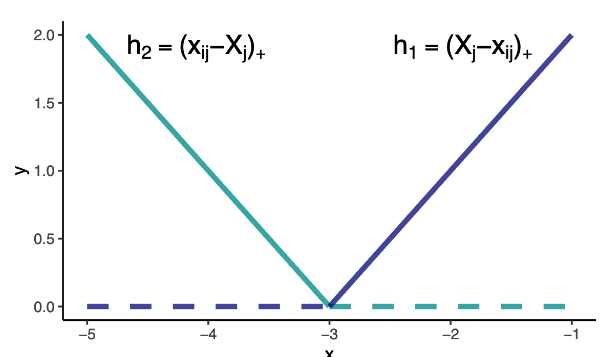
\includegraphics[width=10cm]{Figures/3ref_pair.png}
	\centering
	\caption{The constructed reflected pairs.}
	\label{reflected_pairs}
\end{figure}
So, for each $X_j$, the set of candidate reflected pairs that exist at each of the $x_{ij}$ points of that variable is shown in \green{Figure}~\ref{hinges}. 
\begin{figure}[h]
	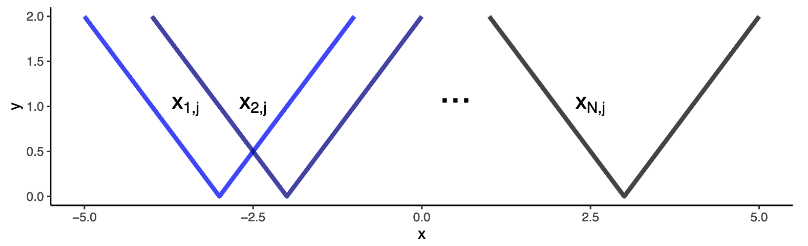
\includegraphics[width=10cm]{Figures/3hinge.png}
	\centering
	\caption{Collections of hinge functions.}
	\label{hinges}
\end{figure}

This means that if all input values are distinct, there are a total of $2Np$ basis functions, and $2N$ divisions in each of the splines for each variable. The model we use to combine all variables is an additive one in $\boldsymbol\beta$:
$$
f(X) = \beta_0 + \sum_{m=1}^M \beta_m h_m(X),
$$
where each function $h_m(X)$ is an element of $\mathcal{C}$ or a linear combination of these basis functions\green{, and $M$ is the number of basis functions included in the model}. For this initial explanation, we will use only functions that do not involve interactions (the model with interactions works very similarly to CART decision trees).

\green{To make the construction concrete, suppose there are $p = 2$ predictors, $x_1$ and $x_2$, each observed $N = 3$ times. The candidate set $\mathcal{C}$ then holds one reflected pair per observation per predictor, twelve basis functions in all. One possible fitted model with no interactions is $\hat f(X) = 2 + 0.5\,(X_1 - 0.3)_+ - 1.2\,(0.7 - X_2)_+$: a flat surface at height two that tilts upward once $x_1$ exceeds $0.3$ and downward as $x_2$ falls below $0.7$. The same two-predictor setting reappears in the next section when basis \textit{types} are introduced, extending this example.}

\green{We write $\mathcal{M}$ for the model itself, understood as the set of basis functions currently included; the construction process that grows $\mathcal{M}$} begins with the base model $\hat f(X) = \hat \beta_0 = h_0(X) = 1$, where a term functioning as an intercept at the origin is defined. To add terms incrementally, all functions in the set $\mathcal{C}$ are candidates for entry into $\mathcal{M}$. For each observation $x_{ij}$, the new model involving these functions is fitted as follows:
$$
\hat f(X) = \hat \beta_0 + \hat \beta_1 h_1(X) + \hat \beta_2 h_2(X).
$$
Since this is a linear form in terms of each of the functions $h_i$, the adjustment of each parameter $\hat \beta_i$ is done by minimizing the sum of squares.

The reflected pair that is added is the one that minimizes the training error. This process is repeated for each of the remaining reflected pairs, solving OLS to determine the new $\boldsymbol\beta$, and adding the one that continues to minimize the error. The stopping criterion can be either that none of the remaining reflected pairs reduces the error enough (in absolute or relative terms) or until we have a predetermined number of variables in the model.

This leads to overfitting the data, but this is the goal in this part of the procedure when minimizing the training error. Once we have $\mathcal{M}$, we start the second part of model fitting, which is the pruning part. In this case, terms $h_i(X)$ are removed iteratively, starting with the one that produces the smallest increase in the residual sum of squares when removed. \green{This backward pass yields, for each model size $\lambda$ (the number of terms retained after pruning), the best model of that size, denoted $\hat f_\lambda$.}

Several procedures can be used to estimate the optimal value of $\lambda$, such as cross-validation or bootstrap, but this involves a significant computational cost. To minimize this cost, MARS models generally use a generalized cross-validation (GCV) procedure. This criterion is defined as:
$$
GCV(\lambda) = \frac{ \sum_{i=1}^N (y_i - \hat f_\lambda(x_i))^2 }{\left( \frac{1 - M(\lambda)}{N} \right)^2},
$$
where the value $M(\lambda)$ is the number of effective parameters in the model, depending on the number of terms plus the number of breakpoints used, penalized by a factor (this factor is 2 in the case for additive in $X$ that we are explaining, and 3 when there are interactions).

Now that we have described the base model, we can go back and consider the differences when incorporating interaction terms. \green{The additive model above has a structural blind spot: because every term depends on a single predictor, the fitted surface can never represent a joint effect, a situation where the influence of one variable depends on the level of another. Interaction terms repair this. An interaction term is a product of hinge functions of different predictors, and it activates only in the region of the input space where all of its factors are positive, which is exactly the local, rectangular kind of joint behaviour that single-variable terms cannot express. The base equation extends naturally: instead of entering the model on its own, a candidate reflected pair may be multiplied into a basis function $h_\ell$ that is already present, so the products between existing terms and candidate pairs become the new candidate terms.} Note that this general case encompasses the previous one because if you want to add a reflected pair without interacting with the other variables, you simply multiply by $h_0 = 1$.

In this way, a model $\mathcal{M}$ with $M$ terms will be updated as follows after finding the combination $\hat \beta_{M+1} h_\ell(X) \cdot \green{(X_j - t)_+} + \green{\hat \beta_{M+2}} h_\ell(X) \cdot (t-X_j)_+$ that best minimizes the training error:
$$
\hat f(X) = \hat \beta_0 + \sum_{m=1}^M \hat \beta_m h_m(X) + \hat \beta_{M+1} h_\ell(X) \cdot (X_j - t)_+ + \hat \beta_{M+2} h_\ell(X) \cdot (t-X_j)_+,
$$
where $h_\ell \in \mathcal{M}$ and $t = x_{ij}$ for any case.

One interesting consideration is that the added flexibility of these models does not end with it being piecewise linear, as one small alteration that can be made is to replace the truncated linear functions with truncated cubic basis functions or other functions of a higher order, which \green{allows} the resulting model to be fully differentiable within its domain. 

In conclusion, our exploration of Multivariate Adaptive Regression Splines (MARS) is a powerful and versatile technique for modelling complex relationships within data. Unlike traditional linear regression, MARS \green{uses} piecewise linear functions, making it a valuable tool when dealing with non-linear relationships between input features and the target variable. The methodology behind MARS involves the creation of reflected pairs and the incremental addition of basis functions to the model, effectively adapting to the data's intricacies. The model construction process aims to minimize the training error by iteratively selecting the reflected pair that provides the most significant reduction in error.

\section{BMARS Models}

The key innovation that distinguishes BMARS from its predecessor lies in its Bayesian framework. While MARS primarily focuses on constructing piecewise linear models by iteratively selecting basis functions to minimize training error, BMARS introduces Bayesian methods to bring a probabilistic perspective into this process. This integration of Bayesian principles allows BMARS to provide not only point estimates of model parameters but also entire probability distributions, enabling a more comprehensive understanding of the uncertainty inherent in the modelling process.

As described in \cite{denison1998bayesian}, which is the original paper where this method was proposed, the idea behind this model is to allow more flexibility in the traditional MARS model by looking at it from a Bayesian perspective. This is done by mimicking the MARS model with changes in framing, namely by considering the number of basis functions, along with their \textit{type}, their coefficients and their form (the positions of the split points and the sign indicators) as random. \green{Concretely, where MARS commits to one set of basis functions with one set of knots and signs, BMARS declares each of these quantities a random variable and places a prior on it. The object of inference is the full configuration of the model: how many basis functions there are, which predictors each one involves, where its knots sit, which direction each hinge opens, and what coefficients multiply the terms. A fitted BMARS is therefore not one spline surface but a posterior distribution over such configurations.} 

We take the definition of a basis type from the original paper and a small example from there to make the definition tangible, and include it here for completeness. 
\begin{definition}
	\green{Let $B_i$ and $B_j$ be two basis functions, and for a basis $B_i$ let $J_i$ denote its degree of interaction, that is, the number of distinct predictors it involves, with $[x(1,i), \ldots, x(J_i,i)]$ the list of those predictors. We consider $B_i$ and $B_j$ to be of the same type if $[x(1,i), \ldots, x(J_i,i)]$ is identical to some permutation of $[x(1,j), \ldots, x(J_j,j)]$. In words, two basis functions share a type exactly when they split on the same subset of predictors, regardless of the order in which those predictors are listed and regardless of knots or signs. Hence, with $m$ predictor variables there are $N$ different types of basis functions, one per nonempty subset of predictors, where $N$ is given by:}
	\begin{equation}
		N = \sum_{i=1}^{m} \binom{m}{i} = 2^m - 1. \label{eq3}
	\end{equation}	
\end{definition}

Note that the sum does not include the constant basis function term (for which $i$ would equal 0 in \eqref{eq3}), as this basis \green{$B_1$} is always the sole constant basis function in the model, so it cannot be chosen as a candidate basis. Frequently, some maximum order of interaction $I$ is assigned to the model, such that $J_i \leq I$ for $i = 1, \ldots, k$. In which case, the sum in \eqref{eq3} only runs from 1 up to $I$. We let $T_i \in \{1, 2, \ldots, N\}$ denote the type of basis function \green{$B_i$}; thus, $T_i$ effectively tells us which predictor variables we are splitting on, i.e., what the values of $x(1,i), \ldots, x(J_i,i)$ are.

\green{To ground this, return to the two-predictor setting of the MARS example, $m = 2$ with predictors $x_1$ and $x_2$. A basis function can involve $x_1$ alone, $x_2$ alone, or both, so there are $2^2 - 1 = 3$ types. Writing $\ast$ as a placeholder for a knot location (whose value does not affect the type), the three shapes are $[\pm (x_1 - \ast)]$ (type 1), $[\pm (x_2 - \ast)]$ (type 2), and $[\pm (x_1 - \ast)][\pm (x_2 - \ast)]$ (type 3). The two example terms $0.5\,(x_1 - 0.3)_+$ and $1.2\,(0.7 - x_2)_+$ from the previous section are then of type 1 and type 2 respectively, and any basis splitting only on $x_2$, whatever its knot or sign, has type 2. The type records which predictors a basis touches and nothing else.}

The key insight that this framework of construction is based on is that any MARS model can be uniquely defined by the following: 
\begin{itemize}
	\item The number of basis functions $k$, 
	\item the coefficients of the basis functions $a_i$, 
	\item the type of basis functions $T_i$, 
	\item the knot points associated with each interacting term $t_{ji}$, 
	\item the sign indicators associated with each interacting term $s_{ji}$. 
\end{itemize}
and as such, a probability distribution over the possible MARS models can be constructed, enabling a more comprehensive understanding of the uncertainty inherent in the modelling process since the response is an entire probability distribution rather than a single model. This framework also provides the ability to do ANOVA and Sobol decompositions for sensitivity analysis. One important aspect of this framework for construction is that the number of parameters varies with the number of basis functions $k$, and as such, a traditional method such as Markov chain Monte Carlo cannot be used directly. An extended version of MCMC is therefore used, called reversible jump MCMC (first introduced in \cite{green1995reversible}), that allows for a variable number of parameters.

\section{BASS Models}

Bayesian Adaptive Spline Surface (BASS) models are an extension of the family of non parametric regression models of which multivariate adaptive regression splines (MARS) was the first developed in 1991 and is the most basic \cite{friedman1991multivariate}. MARS is an extension of linear models, where interactions between variables and non linearities are modelled automatically. 

The extension of this model of interest is the BMARS model. As the authors state in \cite{denison1998bayesian}, the aim of BMARS is to provide a Bayesian model that mimics the MARS procedure. This is done by considering the number of basis functions, along with their type, the coefficients and their form, random. Then, a suitable MCMC algorithm, in this case reversible jump monte carlo \cite{green1995reversible}, is used to \green{approximate the posterior}. The great advantage \green{of} RJMCMC over other MCMC techniques is that the number of parameters can be variable, and as such, is a great basis for the type of analysis that is necessary for models in the MARS class. 

BASS models are an adaptation of BMARS models that include \green{two concrete additions: cheaper reversible-jump proposals that keep posterior sampling efficient at scale, and} parallel tempering for better posterior exploration \cite{francom2020bass}. For our purposes though, the most significant improvement is that it allows the use of categorical variables alongside some continuous variables. This is useful in the context of hyper-parameter optimization, where there are generally some categorical variables such as polynomial degree, smoothing, etc. \green{This capability is exercised directly in this work: the categorical and mixed benchmarks of the experimental chapter are multi-dimensional, and it is what makes BASS applicable to them.} 

A detailed rundown of the model, its priors, and its construction in general can be seen in \cite{francom2020bass}, but, we include the definition of the model presented in that work for completeness. 

Let $y_i$ denote the dependent variable and $\boldsymbol{x}_i$ denote a vector of $p$ independent variables, with $i = 1, \ldots, n$. Without loss of generality, let each independent variable be scaled to be between
zero and one. We model $y_i$ as 
\begin{equation} y_i = f(\boldsymbol{x}_i) + \epsilon_i, \, \, \epsilon_i \sim \mathcal{N}(0,\sigma^2) \label{eq:bass_lik} \end{equation}
\begin{equation} f(\boldsymbol{x}) = a_0 + \sum_{m=1}^{M} a_m B_m(\boldsymbol{x}) \label{eq:bass_f} \end{equation}
\begin{equation} B_m(\boldsymbol{x}) = \prod_{k=1}^{K_m} g_{km} [s_{km}(\boldsymbol{x}_{v_{km}} - t_{km}) ]^\alpha_+ \label{eq:bass_basis} \end{equation}

\green{Equations \eqref{eq:bass_lik} through \eqref{eq:bass_basis} constitute the BASS model: the first is the likelihood, the second the spline representation of the regression surface, and the third the form of each basis function.}

The only difference between this setup and that of MARS and BMARS is the inclusion of the constant $g_{km}$ in each element of the tensor product. This term is $g_{km}=[s_{km}(\boldsymbol{x}_{v_{km}} - t_{km}) ]^\alpha_+$, where $s_{km} \in \{-1,1\}$ is referred to as the sign, $t_{km}\in [0,1]$ is a knot, $v_{km}$ selects a variable, $K_m$ is the degree of interaction, and $\alpha$ determines the degree of the polynomial splines. This normalizes the basis functions so that the basis coefficients $a_1, \ldots, a_M$ are on the same scale, making computations more stable.

The hinge form $[s_{km}(\boldsymbol{x}_{v_{km}} - t_{km})]^\alpha_+$ above is the basis used for \emph{continuous} predictors, and it makes the role of the knot $t_{km}$ a numeric one: it places a slope change at a point along a real axis. This is precisely the construction that does not transfer to a categorical predictor, whose levels have no order and no notion of distance between them. The way BASS resolves this, inheriting the treatment of categorical variables from \cite{friedman1991multivariate} and \cite{denison1998bayesian}, is to use a different kind of factor in the tensor product when the selected variable $\boldsymbol{x}_{v_{km}}$ is categorical: instead of a hinge, the factor becomes an \emph{indicator that the variable's level lies in a chosen subset of its levels}. Formally, if a categorical predictor takes values in a finite set of levels $\mathcal{L}$, the corresponding factor in $B_m(\boldsymbol{x})$ is $\boldsymbol{1}\!\left[\boldsymbol{x}_{v_{km}} \in S_{km}\right]$ for some subset $S_{km} \subseteq \mathcal{L}$. The subset $S_{km}$ plays the role that the knot $t_{km}$ plays for a continuous variable, and like every other element of the model (the number of basis functions, the variables they involve, the knots, and now the level subsets) it is treated as random and explored by the reversible-jump MCMC. Continuous and categorical factors can appear together in the same product $B_m$, so the model represents interactions between the two kinds of variable directly; in the \texttt{BASS} package the maximum order of such categorical interactions is controlled by the \texttt{maxInt.cat} argument, and a predictor is treated as categorical simply by passing it as a factor column \cite{francom2020bass}. This is the mechanism behind the claim made above, and it is what makes BASS able to act as a surrogate over the mixed continuous--categorical search spaces that arise naturally in hyper-parameter optimization, without the encodings that a continuous-only surrogate would require.

\green{Equations \eqref{eq:bass_lik} through \eqref{eq:bass_basis} specify the likelihood and the basis structure, but on their own they are not yet a Bayesian model: what makes the \say{B} of BASS is the prior placed on every quantity that MARS would treat as a fixed choice of the fitting procedure. Following \cite[\S 2]{francom2020bass}, whose treatment descends directly from \cite{denison1998bayesian}, the unknowns are the number of basis functions $M$, the structure of each basis (its degree of interaction $K_m$, the variables $v_{km}$ it involves, the signs $s_{km}$, and the knots $t_{km}$, with level subsets $S_{km}$ taking the place of knots for categorical factors), the coefficients $\boldsymbol{a} = (a_0, a_1, \ldots, a_M)^T$, and the error variance $\sigma^2$. The priors are}
\begin{align}
	M &\sim \text{Poisson}(\lambda), \qquad \lambda \sim \text{Gamma}(h_1, h_2), \label{eq:bass_prior_M}\\
	\boldsymbol{a} \mid \sigma^2, \tau, M &\sim \mathcal{N}\!\left(\boldsymbol{0}, \; \frac{\sigma^2}{\tau} \left(\boldsymbol{B}^T \boldsymbol{B}\right)^{-1}\right), \qquad \tau \sim \text{Gamma}(g_1, g_2), \label{eq:bass_prior_a}\\
	\sigma^2 &\sim \text{InvGamma}(\nu_1, \nu_2), \label{eq:bass_prior_sigma}
\end{align}
\green{where $\boldsymbol{B}$ is the $n \times (M+1)$ matrix of the basis functions evaluated at the data, so that the coefficient prior is a $g$-prior in Zellner's sense, and the structural components of each basis carry independent uniform priors: the degree of interaction $K_m$ uniform on $\{1, \ldots, K_{\max}\}$, the variables $v_{km}$ drawn uniformly without replacement, the signs $s_{km}$ uniform on $\{-1, +1\}$, and the knots $t_{km}$ uniform over the observed range of the selected variable (for a categorical factor, the level subset $S_{km}$ is uniform over the admissible subsets of its levels).}

\green{The posterior over the full configuration,}
\begin{equation}
	p\!\left(M, \lambda, \tau, \{K_m, v_{km}, s_{km}, t_{km}\}_{m=1}^{M}, \boldsymbol{a}, \sigma^2 \;\middle|\; \mathcal{D}\right) \; \propto \; \text{likelihood} \times \text{priors}, \label{eq:bass_posterior}
\end{equation}
\green{is the distribution the reversible-jump sampler targets. Birth moves propose adding a basis function, death moves propose deleting one, and change moves perturb the knots, signs, or variables of an existing one; the $g$-prior structure of \eqref{eq:bass_prior_a} lets the coefficients and variance be integrated out or updated in closed form within each move, which is a large part of what makes the sampler practical. This is where Bayes enters the model of equations \eqref{eq:bass_lik} through \eqref{eq:bass_basis}: every structural decision that MARS makes greedily and once is here a random quantity averaged over its posterior, and the fitted object the sampler returns is the collection of posterior draws over entire spline surfaces that the uncertainty estimation of the next section relies on.}


\section{BASS Models as Surrogates in Bayesian Optimization}

With the discussions of the previous chapter and this one, we now have the tools to use the BASS model as a surrogate. There are a couple of decisions that we have to make though so that the model works properly, discussed in detail in this section. Namely, they are the starting points of the problem, the discretization of the function domain, and how we will handle uncertainty in points that have not yet been evaluated. 

\subsection{Starting Point for the Algorithm}

One common problem with BO is the cold start problem. Basically, it is very difficult for the system to draw inference or make predictions at the beginning of iterations because it simply has no relevant information. Another way of saying this is that the prior in this case is uniform (or discrete uniform depending on the context) over the entire function domain\green{, a statement that quietly presumes the domain is bounded; every search space in this work is a compact box or a finite set of levels, so the uniform reading is well defined here, and on an unbounded domain no such prior would exist}, which is not good. A simple solution to this problem is to give the algorithm a set of starting points in the domain, this could be to either do a small grid search to start for a small number of iterations, or \green{evaluate a small random sample of points to the same end}. Having these few points, then the surrogate has enough information to properly decide a good next point to evaluate with the specific acquisition function selected. The next chapter concerns the experiments that were run to test the potency and viability of this model, and in it, different amounts of starting points are used. Needing the starting points is not something unique to BASS models though, as many other models (for example GPs) also have trouble with cold starts. \green{How the shared initial design is constructed for those experiments is specified in the next chapter.} 

\subsection{Discretization of the Function Domain}

As with any numerical problem, one important step in designing the algorithm to solve it is the discretization of continuous variables. This process involves dividing the continuous input space into discrete intervals or points, enabling the algorithm to operate efficiently within a finite computational framework. The choice of discretization scheme can significantly impact the performance and convergence properties of the optimization process.

One approach to discretization is to define a grid over the input space. This involves partitioning each dimension into a set of equally spaced points, forming a mesh that covers the entire domain. While grid-based discretization offers simplicity and uniformity, it will suffer from the curse of dimensionality, especially in high-dimensional spaces, where the number of grid points grows exponentially with dimensionality.

The way we decided to discretize the space was using Latin Hypercube Sampling (LHS) \cite{mckay2000comparison}. LHS is a statistical sampling method used to generate a set of diverse and representative samples from a multidimensional probability distribution. It is particularly useful in optimization, where obtaining a set of samples that cover the entire parameter space evenly and efficiently is crucial. This method is better for this purpose than a simple grid search or a traditional pseudo-random sample of points generated through Monte Carlo methods. \green{In our setting the distribution in question is nothing exotic: we sample uniformly over the bounded search box, so LHS requires no knowledge of any joint distribution over the parameters. What its stratification buys is even coverage of each coordinate's range, which a plain uniform sample of the same size does not guarantee.} We do not go into too much detail into these methods as they are not the main point of this work, but the interested reader can look to the previously referenced \cite{mckay2000comparison} or \cite{stein1987large}. 

\subsection{Uncertainty Estimation}

At first glance, selecting BASS as the surrogate seems to raise a problem when compared to GPs: a Gaussian process hands us a closed-form predictive mean and variance at any unobserved point, and that variance is exactly what an acquisition function needs in order to decide where to look next, the literal point of Bayesian Optimization. It would appear that a spline-regression surrogate gives us only a point prediction and no such uncertainty. This, however, is not the case, and the reason is that BASS is not a point estimator but a fully Bayesian model. The reversible-jump MCMC does not return a single fitted surface; it returns a sample from the posterior distribution \emph{over surfaces}, that is, a collection of plausible spline models given the data observed so far. Evaluating these retained posterior draws at any candidate point $\boldsymbol{x}$ therefore yields a sample from the posterior predictive distribution of $f(\boldsymbol{x})$, and the spread of that sample is precisely the uncertainty we were worried about. Crucially, this uncertainty is native to the model rather than bolted on after the fact, and it does not assume the predictive distribution is Gaussian, which matters because the BASS posterior predictive is in general a skewed, multi-modal mixture of spline surfaces.

Given these draws, we score a candidate with the same acquisition principle used for the GP baseline, namely Expected Improvement, but computed by Monte Carlo over the posterior samples rather than in closed form. Writing $f_{\text{best}}$ for the best (minimal) value observed so far and $\{f^{(s)}(\boldsymbol{x})\}_{s=1}^{S}$ for the $S$ posterior predictive draws at $\boldsymbol{x}$, the Monte Carlo Expected Improvement is
\[ \widehat{\mathrm{EI}}(\boldsymbol{x}) = \frac{1}{S}\sum_{s=1}^{S} \max\!\left(0,\; f_{\text{best}} - f^{(s)}(\boldsymbol{x})\right), \]
which requires no exploration weight to tune: the exploration--exploitation balance is supplied automatically by the dispersion of the posterior draws. As a cheaper alternative we also implement Thompson sampling, which draws a single surface from the posterior and moves toward its minimizer. Both choices use BASS's own posterior as the source of uncertainty, and because the GP baseline is scored with the same Expected Improvement criterion, the two methods differ only in the surrogate, which is exactly the comparison this work is after. The details of how candidates are generated and scored each iteration are given in the next chapter.
